\subsection{Problem}

\renewcommand{\theequation}{\theenumi}
\begin{enumerate}[label=\thesection.\arabic*.,ref=\thesection.\theenumi]
\numberwithin{equation}{enumi}
	\item Consider a small unit of a factory where there are 5 employees : a supervisor and four labourers. The labourers draw a salary of |5,000 per month each while the supervisor gets |15,000 per month. calculate the mean, median and mode of the salaries of this unit of the factory.\\
	\solution 
	\begin{enumerate}
	\item Finding Mean \\
	\begin{multline}
	\text{Mean salary} = \\\frac{\text{Supervisor's salary} + 4\times \text{Labourer's salary}}{5}
	\end{multline}
	\begin{align}
	\text{Mean salary} &= \frac{15000+5000+5000+5000+5000}{5}
	\end{align}
	$\therefore$ the mean salary is 7000.
	
	\item Finding Median \\
	We need to arrange the salaries in ascending order.Thus we get 5000,5000,5000,5000,15000\\
	Let N = no.of employees = 5\\
	\begin{align}
	\text{Median} &= \brak{\frac{N+1}{2}}^{th} term = 3^{rd}value
	\end{align}
	$\therefore$ the median is 5000.
	
	\item Finding Mode\\
	Mode is the highest occurring frequency of the distribution. 5000 is the most repeating salary.\\
	$\therefore$ Modal salary is 5000.
\begin{comment}	
The following python code computes the area of $\triangle$ABC in Fig.\ref{fig:qfour}.
	\begin{lstlisting}
	./codes/quadrilateral/q4.py
	\end{lstlisting}
	
	
	\begin{figure}[!ht]
	\centering
	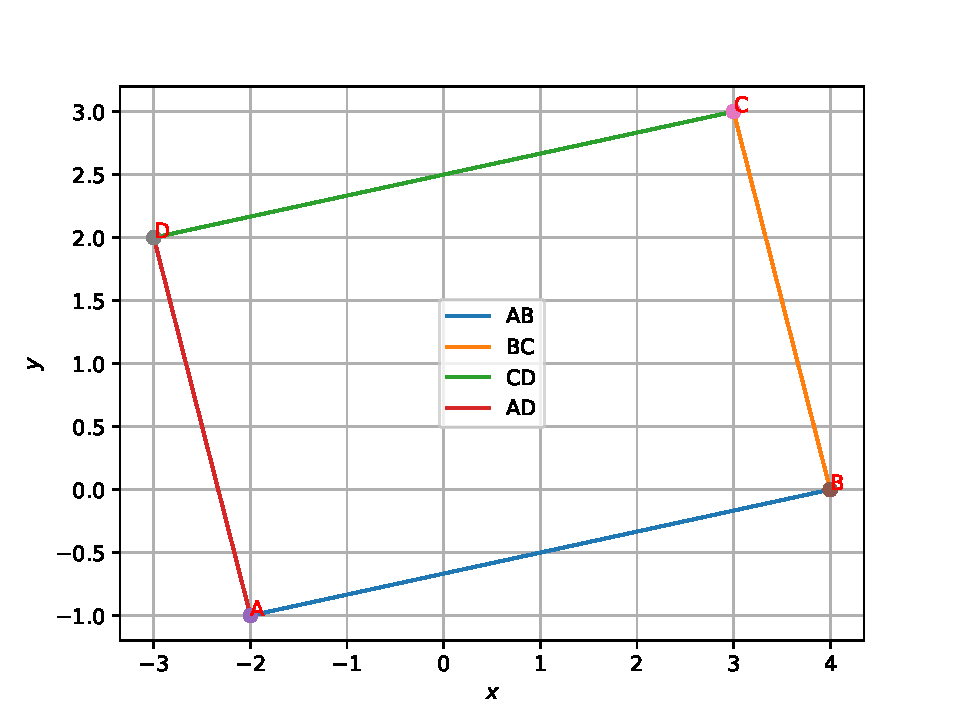
\includegraphics[width=\columnwidth]{./figs/quadrilateral/q4.pdf}
	\caption{Parallelogram of Q.2.2.5}
	\label{fig:qfour}	
	\end{figure}
	
\end{comment}	
\end{enumerate}
\end{enumerate}
